\documentclass[parskip=full]{scrartcl}

\usepackage[utf8]{inputenc}
\usepackage[T1]{fontenc}
\usepackage[ngerman]{babel}
\usepackage{hyperref}
\usepackage{csquotes}

\usepackage{graphicx}
\usepackage{enumitem}
\usepackage{chngcntr}
\usepackage[toc,acronym]{glossaries}
\usepackage{fancyhdr}
\usepackage{float}
\usepackage{caption}
\usepackage{etoolbox}
\usepackage{pdfpages}
\graphicspath{{./resources/}}

\usepackage{implementierungsbericht}

\include{Kapitel/GlossarUndAkronyme}
\makeglossaries

\begin{document}
    \begin{titlepage}

    \begin{center}

        \vspace*{1cm}

            \LARGE
            Testbericht zu

            \Huge
            \textbf{1Sicht}

            \vspace{2cm}

            
\includegraphics[scale=0.4]{/logo/logo_green.jpg}

            \vspace{2cm}
            Erarbeitet von:

            \Large
            \textbf{Hristo Klechorov, Stanimir Bozhilov, Tihomir Georgiev,\\ Martin Zahariev, Maximilian Ackermann\\ und Andry Niclas}

            \vspace{0.3cm}
            \Large
            PSE im Sommersemester 2019\\
            \vspace{0.3cm}
            IPD Reussner und IPD Koziolek\\
            Betreut von: Erik Burger, Sandro Koch und Jan Keim


    \end{center}

\end{titlepage}

    \setcounter{secnumdepth}{5}
    \setcounter{page}{1}

    \tableofcontents

    \pagestyle{fancy}
    \fancyhf{}
    \lhead{1Sicht}

    \chead{
\includegraphics[scale=0.02]{logo/logo_header_black}}

    \cfoot{\thepage}

    \rhead{Einleitung}

\section{Einleitung}

    In diesem Dokument soll es um die Dokumentation der letzten Phase des PSE gehen. Der Fokus lag in dieser Phase vor allem darauf, die Tests aus der Implementierungsphase zu erweitern und eine möglichst hohe Testüberdeckung zu erreichen.
    Zusätzlich dazu haben wir noch andere Arten an Tests geschrieben und eine Umfrage erstellt um andere Leute nach kurzer Benutzung der App nach ihrem Feedback zu fragen.


    \rhead{Zeitplan}

\section{Zeitplan}

    \subsection{Geplanter Zeitplan}

        Der Folgende Zeitplan zeigt die geplante Durchführung der Implementierungsphase. Die einzelnen Meilensteine haben wir dabei nach packages aufgeteilt.

        Durch den Bottom-Up Ansatz bei der Implementierung der Server packages, von database, über repository bis zu den controller, ließ sich gerade diese Phase der Implementierung gut planen.

        Bei der Client-App gab es den Vorteil, dass sich die Implementierung der UI von der der datenhaltenden packages trennen ließ.

        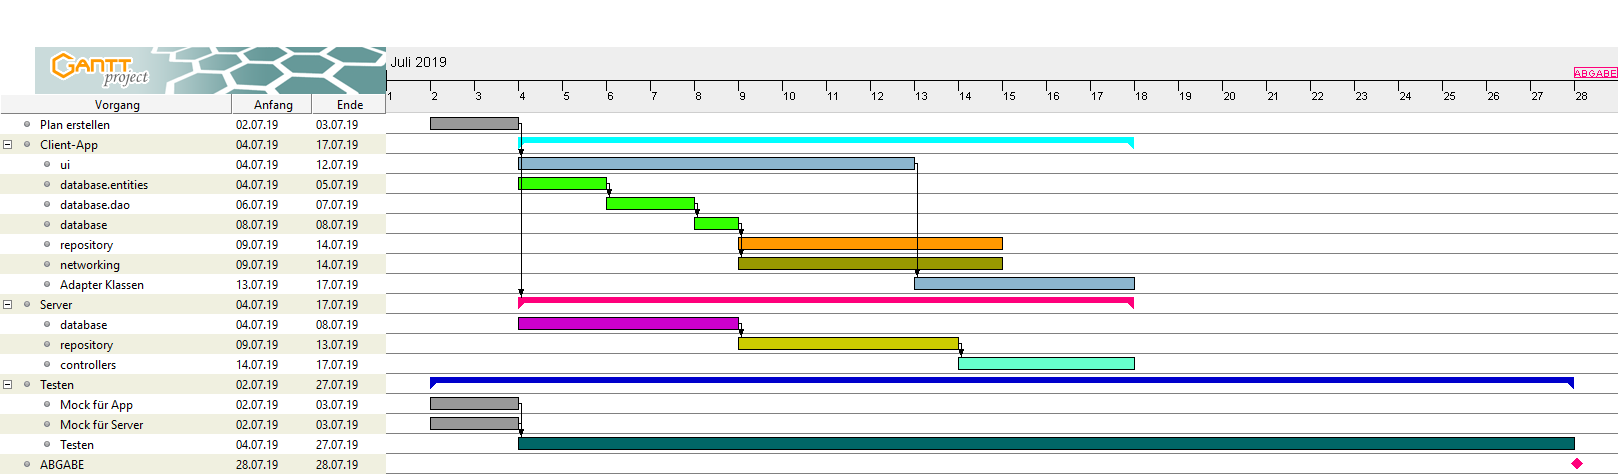
\includegraphics[angle = 90, scale = 0.38]{planung/ganttdiagrammplan.png}

    \subsection{Tatsächlicher Zeitplan}

        Durch verschiedene Verzögerungen bei der Implementierung, auf die später noch genauer eingegangen wird, und durch die zwei Wochen Klausurenphase ergab sich dann folgender Zeitplan:

        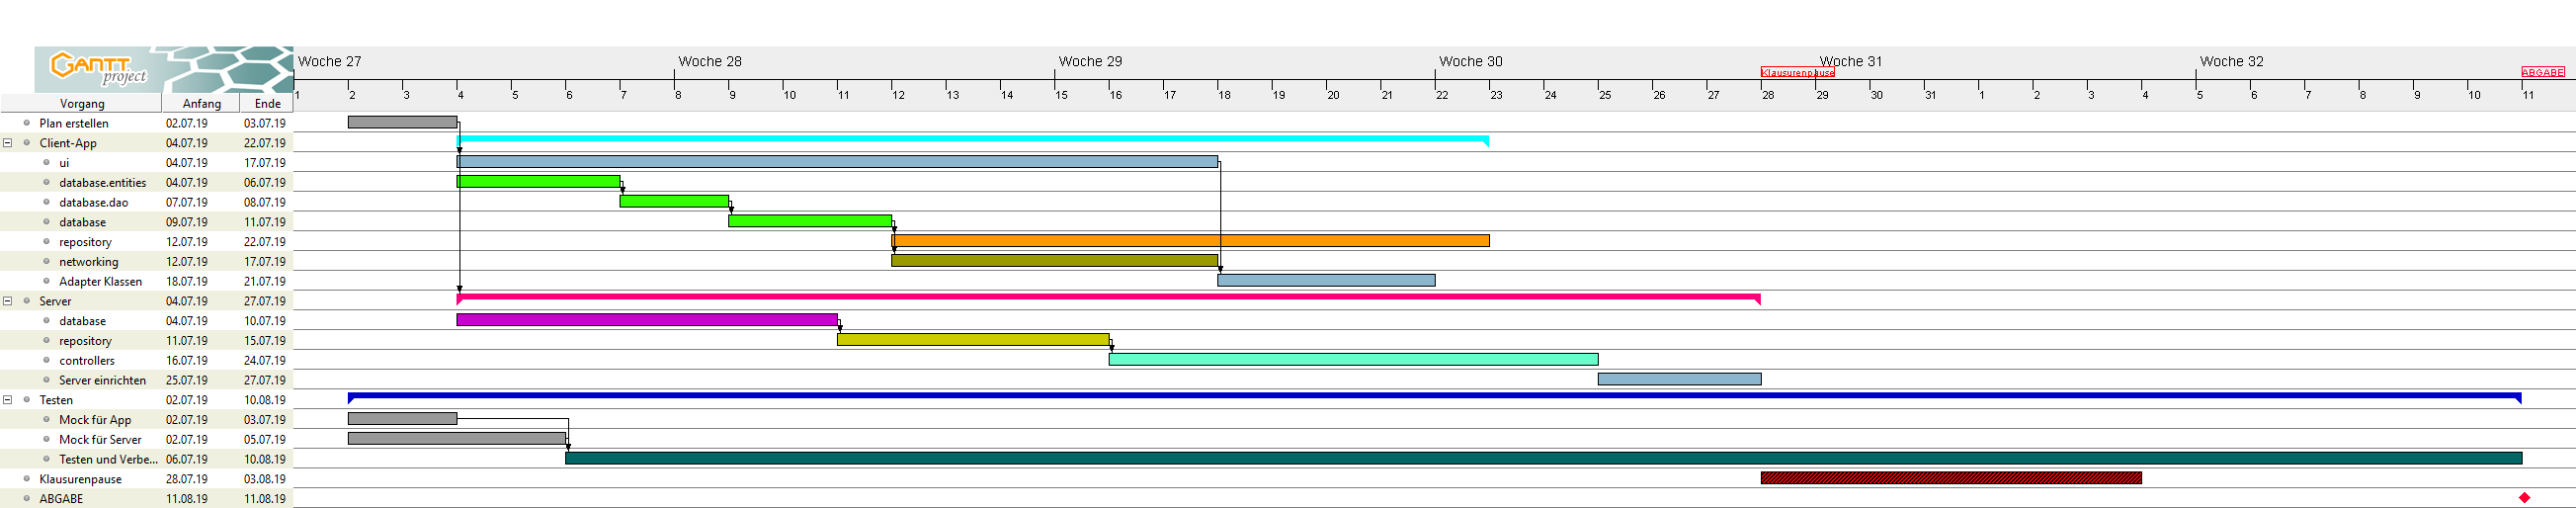
\includegraphics[angle = 90, scale = 0.23]{planung/ganttdiagrammactual.png}


    % \rhead{Wunschkriterien}

\section{Wunschkriterien}

    \subsection{Implementierte Wunschkriterien}

    \subsection{Geänderte und nicht implementierte Wunschkriterien}


    \rhead{Änderungen an der Client-App}

\section{Änderungen an der Client-App}

    In diesem Kapitel werden die Unterschiede der Implementierung, im Gegensatz zum ursprünglichem Entwurf, genauer erklärt.

    \subsection{create-Methoden in den repository-Klassen}

        Im Entwurf war es noch so geplant, dass die Klassen im repository-package die Objekte zwischen der lokalen Datenbank der App und der Datenbank des Servers verwaltet. Dies sollte zum Beispiel das Einfügen und Aktualisierung von Objekten beinhalten.

        Wir haben uns jedoch frühzeitig dazu entschieden, dass diese Klassen auch die Erstellung der Objekte übernehmen sollen. Dadurch werden zum Beispiel viele extra Aufrufe vermieden, welche Überprüfen ob ein bestimmtes Objekt schon existiert. Dies kann nun intern in den repository-Klassen geschehen, mit Hilfe von einer create Methode in jeder der entsprechenden Klasse.

    \subsection{task-package}

         Um die Daten im Hintergrund zu verarbeiten, damit der Nutzer die App weiter verwenden kann, ohne auf die Daten zu warten, haben wir ein neues package im repository-package erstellt.
         Dieses task-package enthält für jede Dao-Klasse eine Klasse, die mit Hilfe von AsyncTasks die jeweiligen Operationen der Daos im Hintergrund ausführt.

    \subsection{networking-package}

        Laut dem Entwurf sollten die Methoden in den Service-Klassen Objekte oder Listen an Objekten zurückgeben. Dies würde jedoch zu Problemen führen, sollte die App auf eine Antwort des Servers warten.
        Mit Hilfe der Observables kann die App nun weiterlaufen, ohne auf die Antwort zu warten.

    \newpage

    \subsection{utils-package}

        Es wurde im ui-package ein weiteres package mit den Adapter-Klassen, die im Entwurf im ui/shared-package zu finden waren, und weiteren Klassen angelegt:

        Einmal die CustomApp-Klasse um die Funktionalitäten der LocaleHelper-Bibliothek zu verwenden.
        Auch für die Umsetzung der Funktionalitäten dieser Bibliothek wurde die Klasse BaseActivity gebraucht.

        Um generell die Adapter in Views darzustellen und doppelten Code in den Adaptern selbst zu vermeiden, wurde die Klasse BaseViewHolder geschrieben, welche einen beliebigen Adapter an sich bindet und den Inhalt darstellt.

        Des weiteren wurden die Employee- und Student-Adapter Klassen zu einer einzelnen UserAdapter-Klasse zusammengeführt.
        Außerdem wurde der RequestsAdapter hinzugefügt, um die Bestätigungsanfragen der Mitarbeiter einem Administrator anzuzeigen und der ReviewAdapter um Klausureinsichten den Mitarbeitern und Administratoren anzuzeigen.

    \subsection{entities-package}

        Die Klassen im entities-package wurden auch verändert, damit das Verschicken und Empfangen von Gson Objekten vom und zum Server funktioniert.

    \subsection{nullable Variablen}

        Generell gab es diese Variablen, welche auch als nullable implementiert werden sollten, jedoch nicht im Entwurf so beschrieben wurden.


    \rhead{Änderungen am Server}

\section{Änderungen am Server}

    In der tatsächlichen Implementierung ließ sich der Entwurf ohne Änderungen übernehemen.


    \rhead{Implementierung der Client-App}

\section{Implementierung der Client-App}

    In diesem Kapitel wird die Implementierung der Client-App beschrieben. Des Weiteren wird auf die aufgetretenen Schwierigkeiten eingegangen, aber auch auf die Dinge, die sich leichter umsetzen ließen als gedacht.

    \subsection{Generelles zur Implementierung}

        \subsubsection{Implementierung der Activities}

            Zuerst wurden die größten Activities einzeln für sich erstellt, wie etwa die LoginActivity oder die ReviewCreationActivity. Das führte dazu, dass man früh schon die einzelnen Activites benutzen konnte, um deren Implementierung für sich zu testen.

    \subsection{Schwierigkeiten bei der Implementierung}

        \subsubsection{Sprachänderung}

            Die Änderung der Nutzersprache für jeden Nutzer dauerte länger, da es zur Laufzeit geschehen sollte, und nicht eine andere Version der App beim Download runtergeladen wird.
            Um das nun doch zu ermöglichen benutzen wir jetzt eine Bibliothek und konnten nicht einfach nur die Werte aus der .xml laden.

        \subsubsection{Probleme mit Zeitstamps}

            Da es bei den Klassen FOO und BAR zu Problemen mit den Zeitstamps kam, musste im database-package noch die Klasse Converters implementiert werden, um die long-Variablen in Timestamp-Variablen umzuwandeln.


    \rhead{Implementierung des Servers}

\section{Implementierung des Servers}

    In diesem Kapitel wird die Implementierung des Servers beschrieben. Des Weiteren wird auf die aufgetretenen Schwierigkeiten eingegangen, aber auch auf die Dinge, die sich leichter umsetzten ließen als gedacht.

    \subsection{Generelles zur Implementierung}

        Bei der Implementierung der Geschäftslogik des Servers selbst stieß man auf wenigere Probleme, da es sich dabei quasi nur um Kotlin-Code handelt. Die Teile des Servers die sich jedoch um Konnektivität und andere Ktor-abhängige Abläufe gekümmert haben, dauerten deutlich länger zu implementieren, wie es auch noch im späteren Verlauf dieses Kapitels beschrieben wird.

    \subsection{Schwierigkeiten bei der Implementierung}

        \subsubsection{Gehosteter Server}

            Als Host für den Server hatten wir uns für BW-Cloud entschieden. Zum einen auf die Empfehlung der Betreuer, zum anderen da der Dienst kostenlos ist.
            In den letzten zwei Wochen der Implementierungsphase ist dieser Server jedoch mehrmals abgestürzt, ohne das wir eine Möglichkeit gesehen haben den Fehler zu beheben. Dies führte dazu, dass wir jedes Mal eine neue Instanz anlegen und einrichten mussten.

        \subsubsection{Generelle Verzögerungen}

            Da es sich bei Ktor um ein relativ neues Framework handelt, gab es zwar Dokumentation zu der Verwendung, jedoch war es eher schwierig weitere Antworten auf Fragen, in Form von YouTube-Videos oder StackOverflow-Beiträgen zu finden.
            Das führte dazu, dass sie die Implementierung des Servers verzögerte, da man viele Dinge durch Trial-and-Error herausfinden musste und mehrmals die Dokumentation lesen musste, um diese voll zu verstehen.


    \rhead{Tests}

\section{Tests}

    In diesem Kapitel soll es um die verschiedenen Arten von Tests gehen, die wir eingesetzt haben um unsere App zu testen.

    \subsection{JUnit Tests}

        Mit Hilfe von JUnit Tests wurde die Geschäftslogik der App und des Servers getestet. Diese unterschieden sich von den Tests die wir bereits in der Implementierungsphase geschrieben haben nur in sofern, dass sie mehr Zeilen im Code überdeckt haben.

    \subsection{Espresso Tests}

        Espresso Tests gehören zu den UI-Tests, die wir geschrieben haben, um Bugs bei der UI der App zu finden. Bei diesen Tests wird mithilfe eines Emulators ein Android-Gerät simuliert, und bestimmte Buttons und Eingaben festgelegt, die während des Ablaufs des Tests simuliert werden.
        Dabei können auch andere Variablen getestet werden, um die Funktion sicherzustellen.

    \subsection{Manuelle Tests}

        Während der Phase haben wir die App auch immer wieder manuell getestet, da dies einfacher und schneller war als Espresso-Tests zu schreiben. Dies eignete sich vor allem am Anfang, um ein genaueres Gefühl für die Art an Bugs zu bekommen, die bei unserer App häufiger vorkamen.
        Dazu gehörten vor allem das Wechseln von Activities und die Aktionen von Buttons auf dem Screen und die Android-(Hardware-) Buttons.
        Sollte jemand einen Bug dadurch finden, wurde er nummeriert und mitsamt Beschreibung und möglichem Lösungsansatz auf unserem internen Discord-Server gepostet.


    % \rhead{Glossar}
    % \printglossary[nonumberlist]

    % \newpage

    % \rhead{Akronyme}
    % \printglossary[type = \acronymtype, nonumberlist]

\end{document}
